\documentclass[t,xcolor={usenames,dvipsnames}]{beamer}

\mode<presentation>
{
\usetheme{Frankfurt}%{Warsaw}
%\setbeamercovered{transparent}
%\setbeamercolor{background canvas}{bg=white}
}

% Delete these, if you do not want the table of contents to pop up at
% the beginning of each (sub)section:
%\AtBeginSubsection[]
%{
%  \begin{frame}<beamer>{Outline}
%    \tableofcontents[currentsection,currentsubsection]
%  \end{frame}
%}
%\AtBeginSection[]
%{
%  \begin{frame}<beamer>{Outline}
%    \tableofcontents[currentsection]
%  \end{frame}
%}

\usepackage[english]{babel}
\usepackage[latin1]{inputenc}
\usepackage{times}
\usepackage[T1]{fontenc}
\usepackage{verbatim}
\usepackage{url}
\usepackage{amsmath,amssymb}
\usepackage{comment}
\usepackage{hyperref}

% Author-date citations
\usepackage[authoryear,round]{natbib}
\let\cite=\citep  % default \cite such as {\LaTeX} authors are used to

% Where \includegraphics should look for figures
\graphicspath{{./figs/}}
\usepackage{epstopdf}
\DeclareGraphicsExtensions{.eps,.png,.jpg,.pdf}

% Shortcuts
\newcommand{\myhref}[2]{\href{#1}{\textcolor{Blue}{#2}}}
\newcommand{\subitem}[1]{\begin{itemize}[<.->]\item #1 \end{itemize}}
\newcommand{\ghead}[1]{{\tiny #1\\}}
\newcommand{\doi}[1]{\myhref{http://dx.doi.org/#1}{doi:#1}}
\newcommand{\csym}[1]{\textcolor{Blue}{\texttt{#1}}}


%%%%%%%%%%%%%%%%%%%%%%%%%%%%%%%%%%%%%%%%%%%%%%%%%%%%%%%%%%%%%%%%%%%%%%
\title{Functional Curation of Cardiac Cellular Models}
\author{Jonathan Cooper}
\institute[University of Oxford]
{Computational Biology Group\\
 Department of Computer Science\\
 University of Oxford}

\begin{document}

\begin{frame}
\titlepage
\end{frame}

%%%%%%%%%%%%%%%%%%%%%%%%%%%%%%%%%%%%%%%%%%%%%%%%%%%%%%%%%%%%%%%%%%%%%%

\begin{frame}{Outline}
\setcounter{tocdepth}{1}
\tableofcontents
\end{frame}

%%%%%%%%%%%%%%%%%%%%%%%%%%%%%%%%%%%%%%%%%%%%%%%%%%%%%%%%%%%%%%%%%%%%%%
\section{A brief history of me}
\subsection*{Main}
%%%%%%%%%%%%%%%%%%%%%%%%%%%%%%%%%%%%%%%%%%%%%%%%%%%%%%%%%%%%%%%%%%%%%%
% Start with personal slides v quickly as last done 2009/02/11 !

\begin{frame}{1983 --- Tooting Bec, London}
\begin{columns}[T]
\column{.5\linewidth}
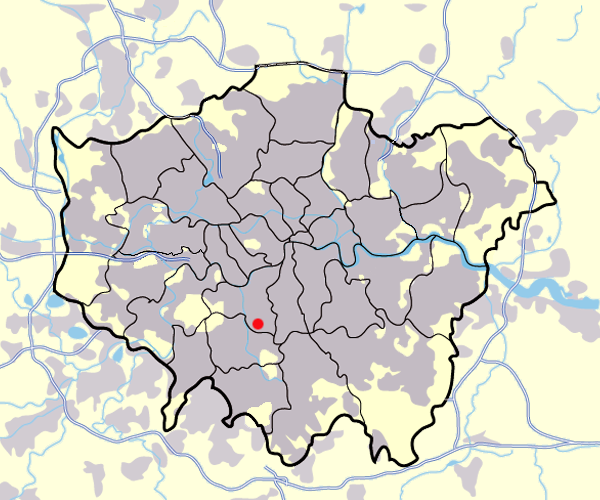
\includegraphics[width=.9\textwidth]{LondonMap}
\column{.5\linewidth}
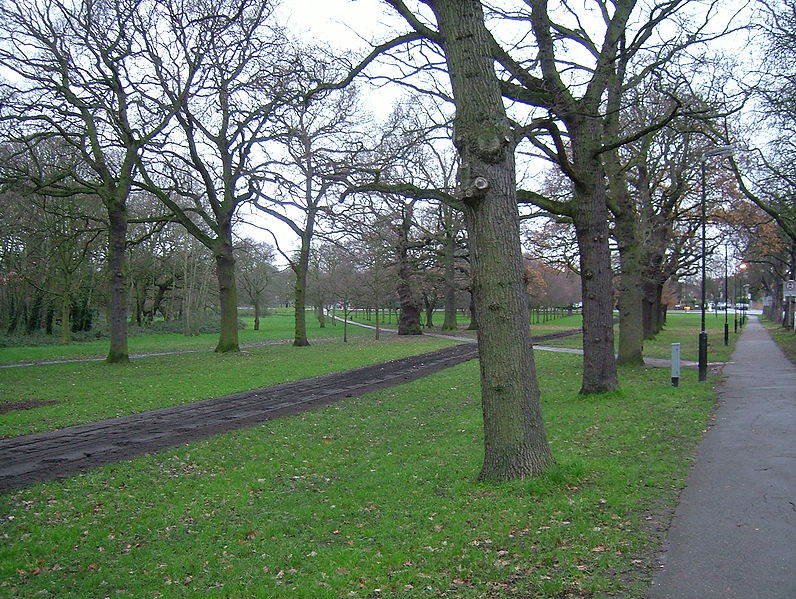
\includegraphics[width=.9\textwidth]{TootingBecCommon}
\end{columns}
\end{frame}

\begin{frame}{1987 --- Zambia, Africa}
\vspace{-1cm}
\begin{columns}[T]
\column{.5\linewidth}
\begin{center}
\only<1>{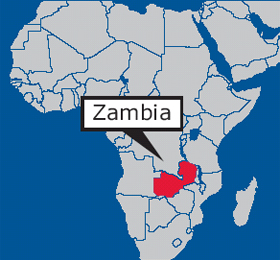
\includegraphics[width=.9\textwidth]{ZambiaMap}}
\only<2>{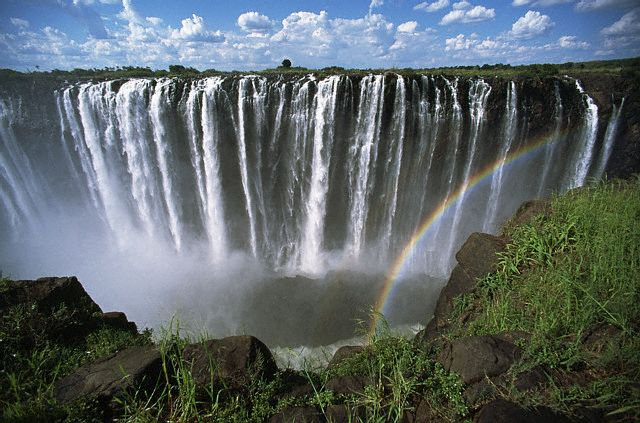
\includegraphics[width=.9\textwidth]{VictoriaFalls}\\
\vspace{.2cm}
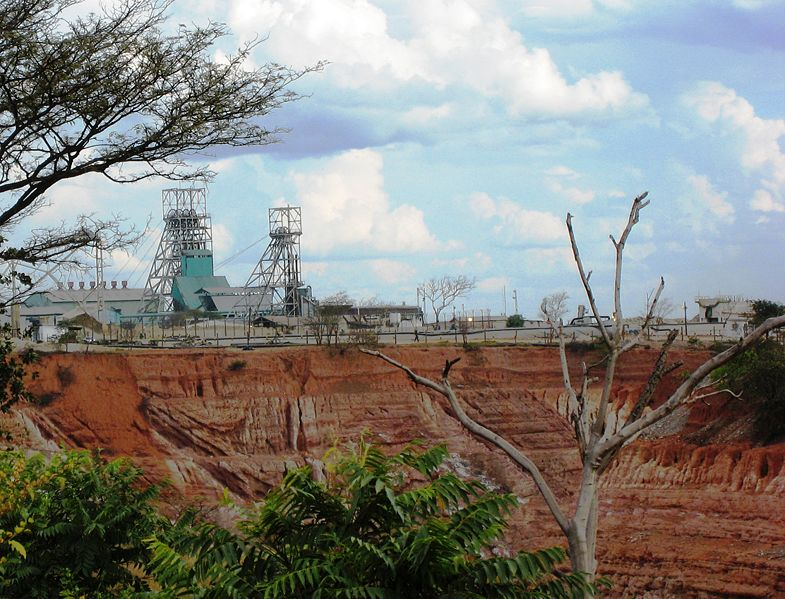
\includegraphics[width=.9\textwidth]{KitweCopperMine}}
\end{center}
\column{.5\linewidth}
\begin{center}
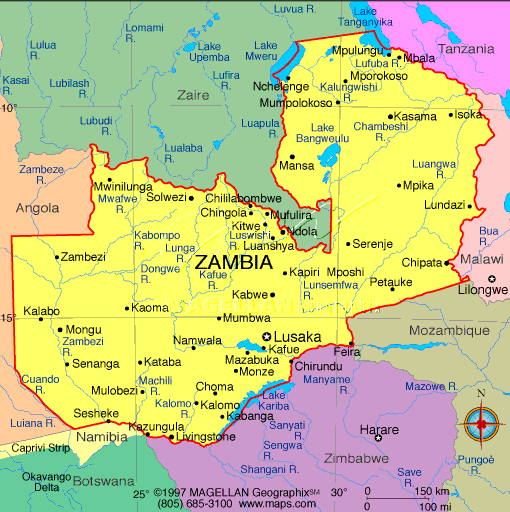
\includegraphics[width=.85\textwidth]{zambia}\\
\only<2>{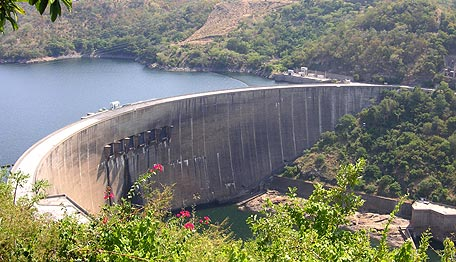
\includegraphics[width=.9\textwidth]{KaribaDam}}
\end{center}
\end{columns}
\end{frame}

\begin{frame}{1993 --- Back to England}
\begin{center}
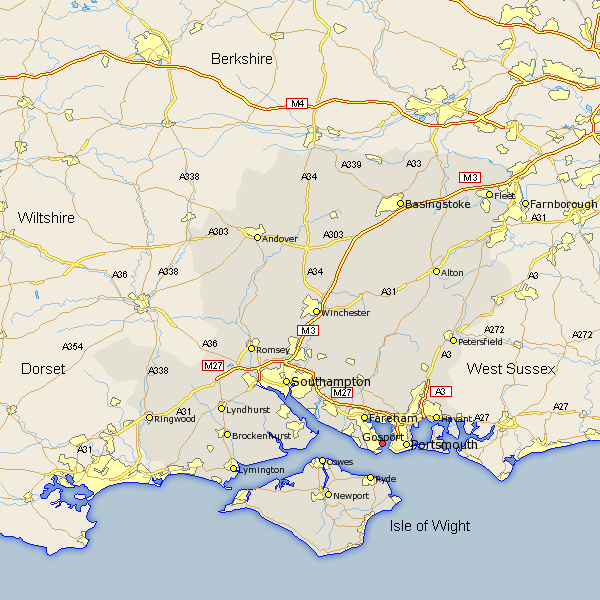
\includegraphics[height=.8\textheight]{GosportMap}
\end{center}
\end{frame}

\begin{frame}{2001 --- Oxford}
\begin{columns}[T]
\column{.35\linewidth}
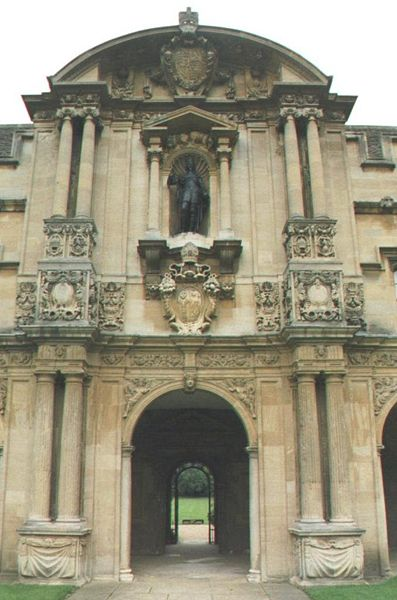
\includegraphics[width=.99\textwidth]{sjc1}
\column{.6\linewidth}
\hspace{.05\textwidth}
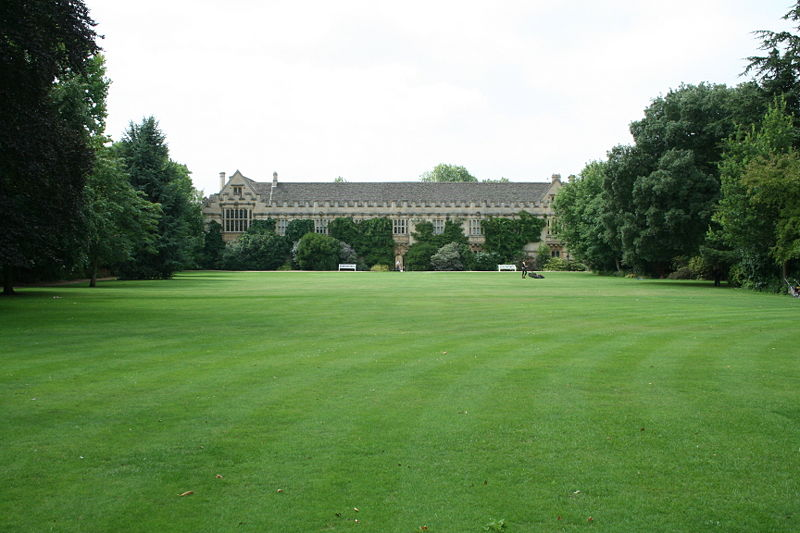
\includegraphics[width=.9\textwidth]{sjc2}
\begin{itemize}
\item 2001: BA, Mathematics \& Computer Science
\item 2004: DPhil, LSI DTC \& Computing Laboratory
\item 2008: Various postdocs
\end{itemize}
\end{columns}
\end{frame}

%%%%%%%%%%%%%%%%%%%%%%%%%%%%%%%%%%%%%%%%%%%%%%%%%%%%%%%%%%%%%%%%%%%%%%
\section{Introduction to functional curation}
\subsection*{Main}
%%%%%%%%%%%%%%%%%%%%%%%%%%%%%%%%%%%%%%%%%%%%%%%%%%%%%%%%%%%%%%%%%%%%%%
% * Explain problem, focus on sell, ability to describe and run a variety of experiments
% * Outline functional curation, demonstrate 2 example protocols

\begin{frame}{What is the problem?}
\begin{itemize}
\item Many (cardiac cell) models exist
  \begin{itemize}
  \item Multiple models of a system are developed to explore and compare hypotheses
  \item How do we choose between them?
  \end{itemize}
\item What functionality does a model have?
\item How do we robustly parameterise models and challenge them with data?
\item How can we determine a model's limitations or suitability for a given study?
\item When extending a model to explore a new experimental scenario, does it still reproduce the original behaviour?
\end{itemize}
\end{frame}

\begin{frame}{Models and experiments}
\begin{itemize}
\item We have languages (e.g.\ CellML) to describe mathematical models
\item Models are based on and tested by \alert{experiments}
\item We are developing
  \begin{itemize}
  \item A \alert{protocol language} to describe experiments
  \item A tool to run these on models and compare results
  \end{itemize}
\end{itemize}
\end{frame}

\begin{frame}{Potential applications}
\begin{itemize}
\item Rational model selection: based on ability to produce expected results for set of protocols
  \subitem{Or motivate further development if none can}
\item Explore which model features are essential for particular behaviours
\item ``Test-driven'' model development: continual comparison to set of protocols and experimental data
  \subitem{Build up a published library thereof}
\item Parameter fitting to a set of protocols
\item Parameter sweeps, sensitivity analysis, \ldots
\end{itemize}
\end{frame}

\begin{frame}{Example: S1-S2 restitution}
\begin{center}
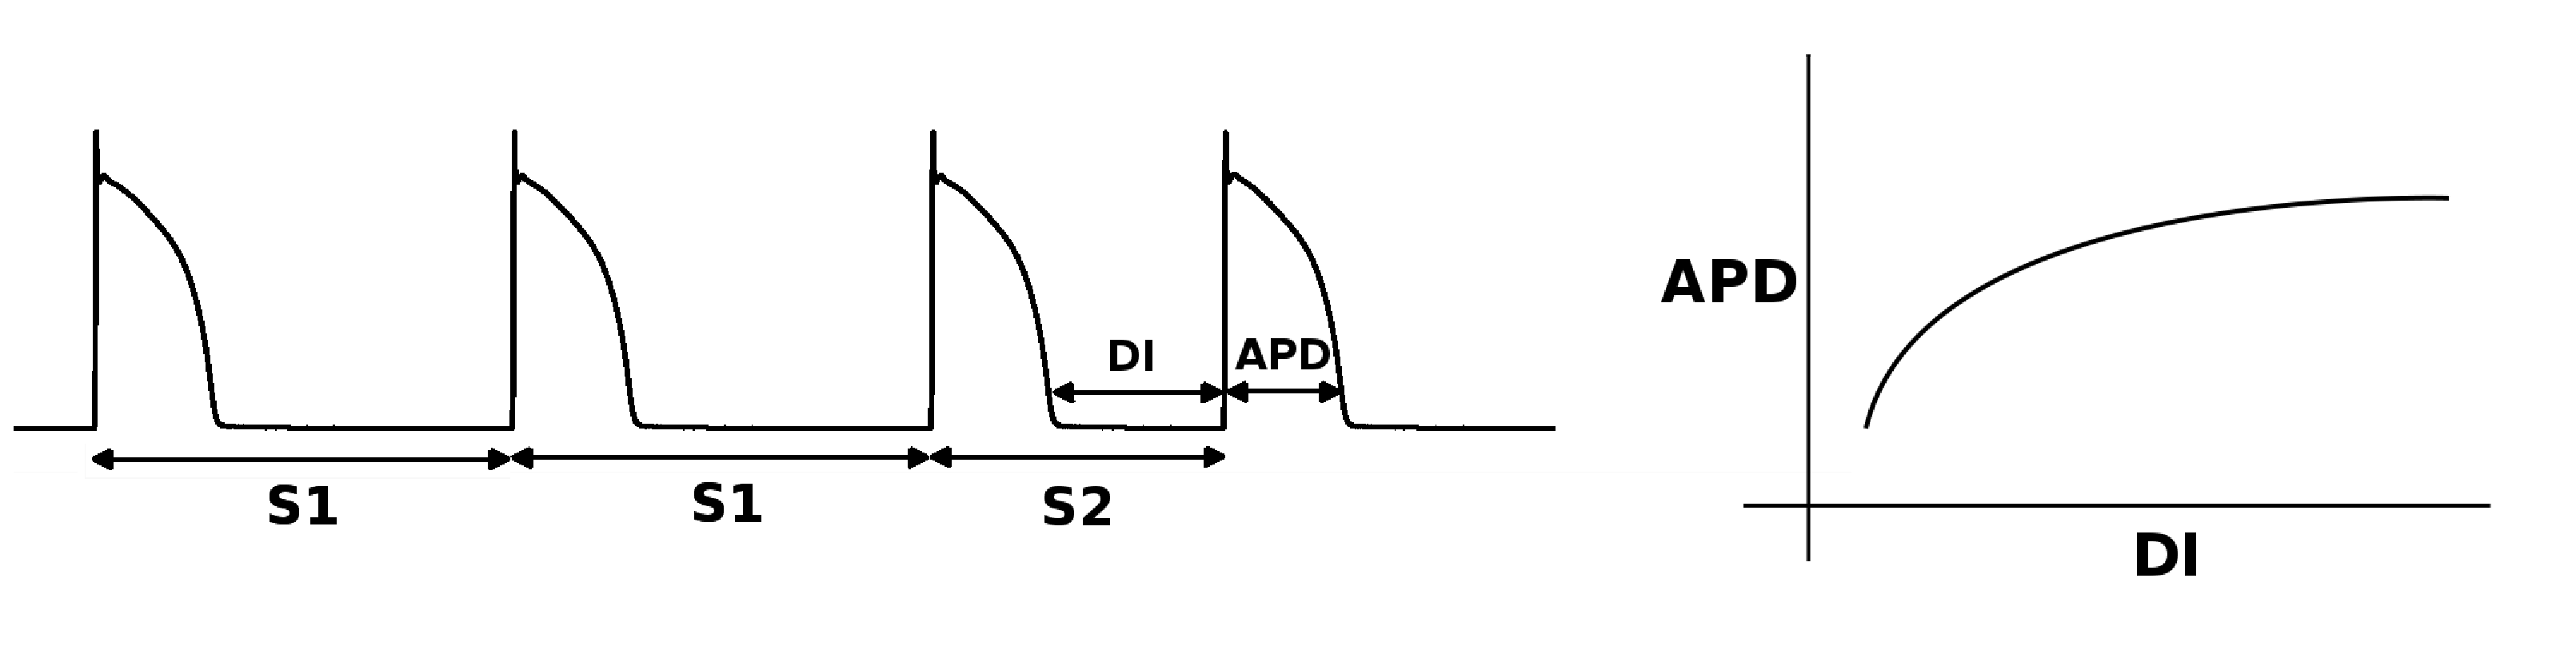
\includegraphics[width=\textwidth]{S1S2}
\end{center}
\end{frame}

\begin{frame}{Example: S1-S2 restitution on canine models}
\begin{columns}[T]
\begin{column}{.33\linewidth}
\begin{center}
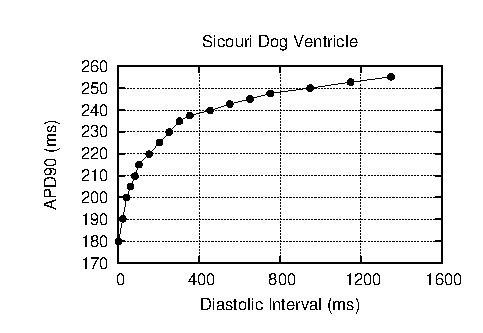
\includegraphics[width=\textwidth]{sicouri_dog_ventricle_s1s2_curve}\\
\vspace{.1cm}
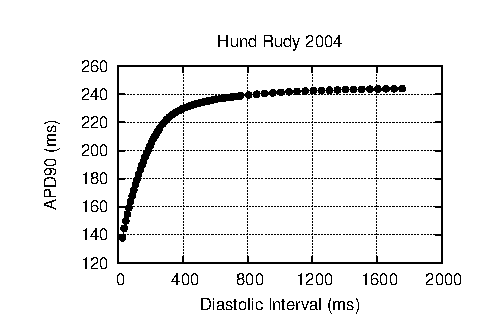
\includegraphics[width=\textwidth]{hund_rudy_2004_s1s2_curve}
\end{center}
\end{column}
\begin{column}{.33\linewidth}
\begin{center}
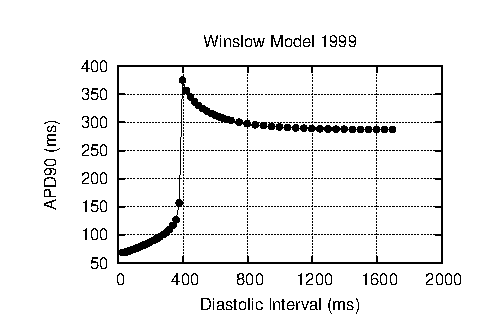
\includegraphics[width=\textwidth]{winslow_model_1999_s1s2_curve}\\
\vspace{.1cm}
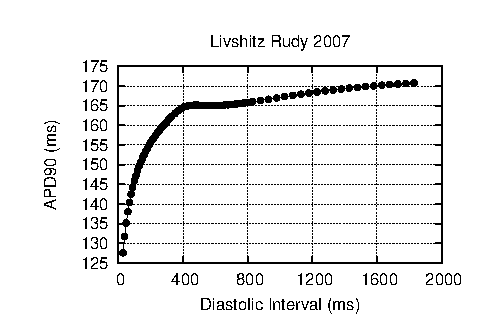
\includegraphics[width=\textwidth]{livshitz_rudy_2007_s1s2_curve}
\end{center}
\end{column}
\begin{column}{.33\linewidth}
\begin{center}
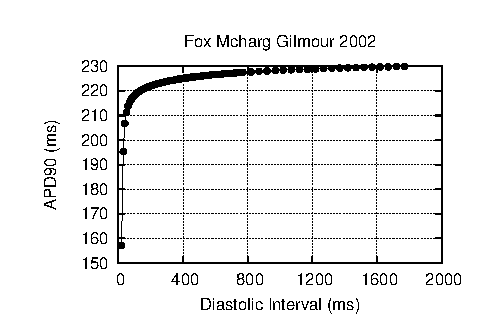
\includegraphics[width=\textwidth]{fox_mcharg_gilmour_2002_s1s2_curve}\\
\vspace{.1cm}
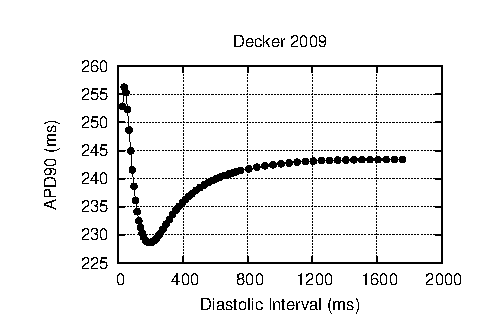
\includegraphics[width=\textwidth]{decker_2009_s1s2_curve}
\end{center}
\end{column}
\end{columns}
\end{frame}

\begin{frame}{Example: S1-S2 restitution on human models}
\begin{columns}[T]
\begin{column}{.33\linewidth}
\begin{center}
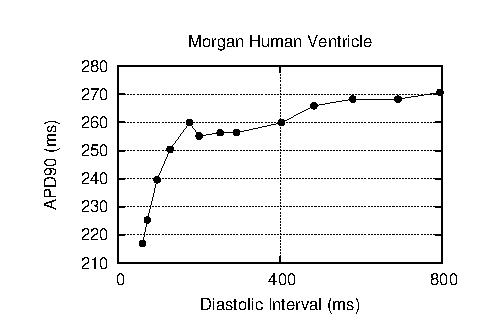
\includegraphics[width=\textwidth]{morgan_human_ventricle_s1s2_curve}\\
\vspace{.1cm}
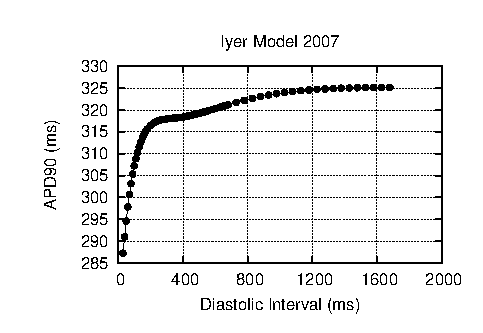
\includegraphics[width=\textwidth]{iyer_model_2007_s1s2_curve}
\end{center}
\end{column}
\begin{column}{.33\linewidth}
\begin{center}
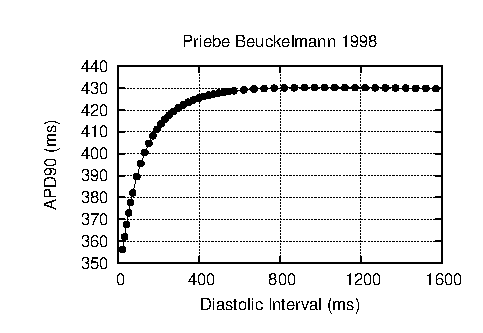
\includegraphics[width=\textwidth]{priebe_beuckelmann_1998_s1s2_curve}\\
\vspace{.1cm}
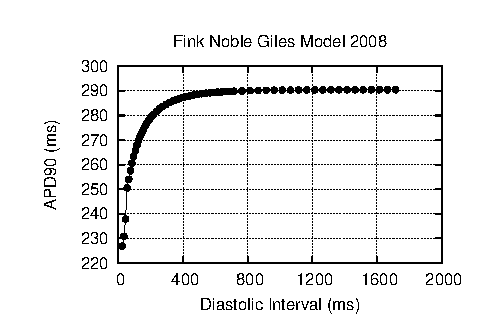
\includegraphics[width=\textwidth]{fink_noble_giles_model_2008_s1s2_curve}
\end{center}
\end{column}
\begin{column}{.33\linewidth}
\begin{center}
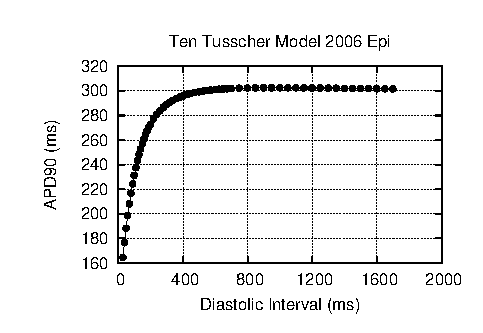
\includegraphics[width=\textwidth]{ten_tusscher_model_2006_epi_s1s2_curve}\\
\vspace{.1cm}
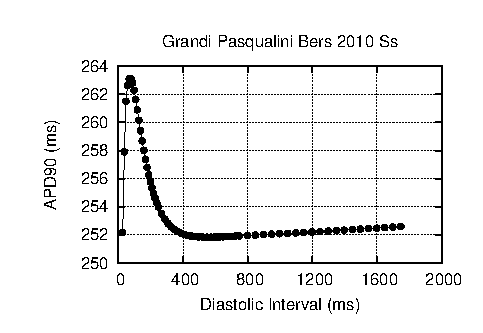
\includegraphics[width=\textwidth]{grandi_pasqualini_bers_2010_ss_s1s2_curve}
\end{center}
\end{column}
\end{columns}
\end{frame}

\begin{frame}{Example: $I_{\textrm{Ca}_L}$ voltage clamp}
\begin{center}
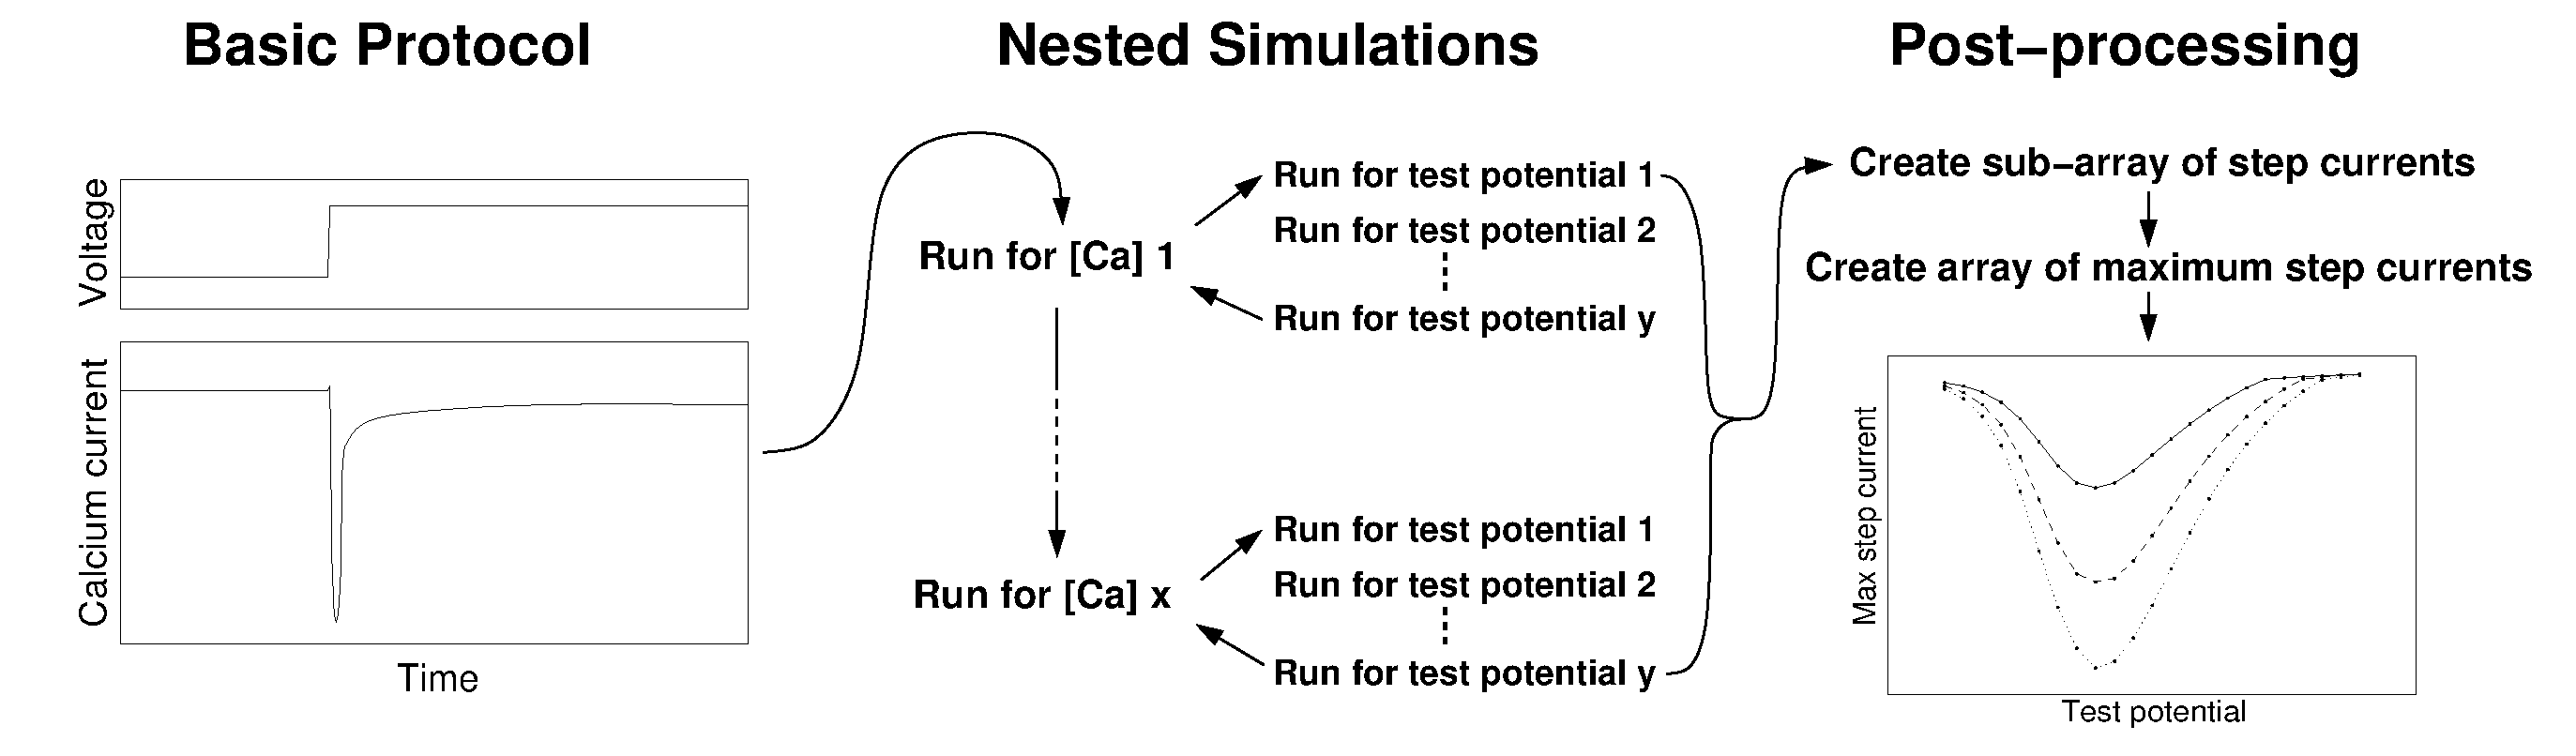
\includegraphics[width=\textwidth]{ICaLIntro}
\end{center}
\end{frame}

\begin{frame}{Example: $I_{\textrm{Ca}_L}$ voltage clamp}
Any suggestions for nice models to show?
Include Corrias, Bondarenko.
\end{frame}

%%%%%%%%%%%%%%%%%%%%%%%%%%%%%%%%%%%%%%%%%%%%%%%%%%%%%%%%%%%%%%%%%%%%%%
\section{Protocol language details}
\subsection*{Main}
%%%%%%%%%%%%%%%%%%%%%%%%%%%%%%%%%%%%%%%%%%%%%%%%%%%%%%%%%%%%%%%%%%%%%%

\begin{frame}{What goes in a protocol?}
\begin{itemize}
\item Definition of the interface with the model being experimented on
\item Definition of simulations to perform
\item Post-processing operations on simulation results
\item Description of what to plot
\item ``Extra bits''
  \begin{itemize}
  \item Inputs to the protocol
  \item Library of functions and/or variables
  \item Specify protocol outputs of interest
  \item Imports of other protocols
  \end{itemize}
\end{itemize}
\end{frame}

\begin{frame}{Protocol structure}
\begin{center}
\vspace{-.5cm}
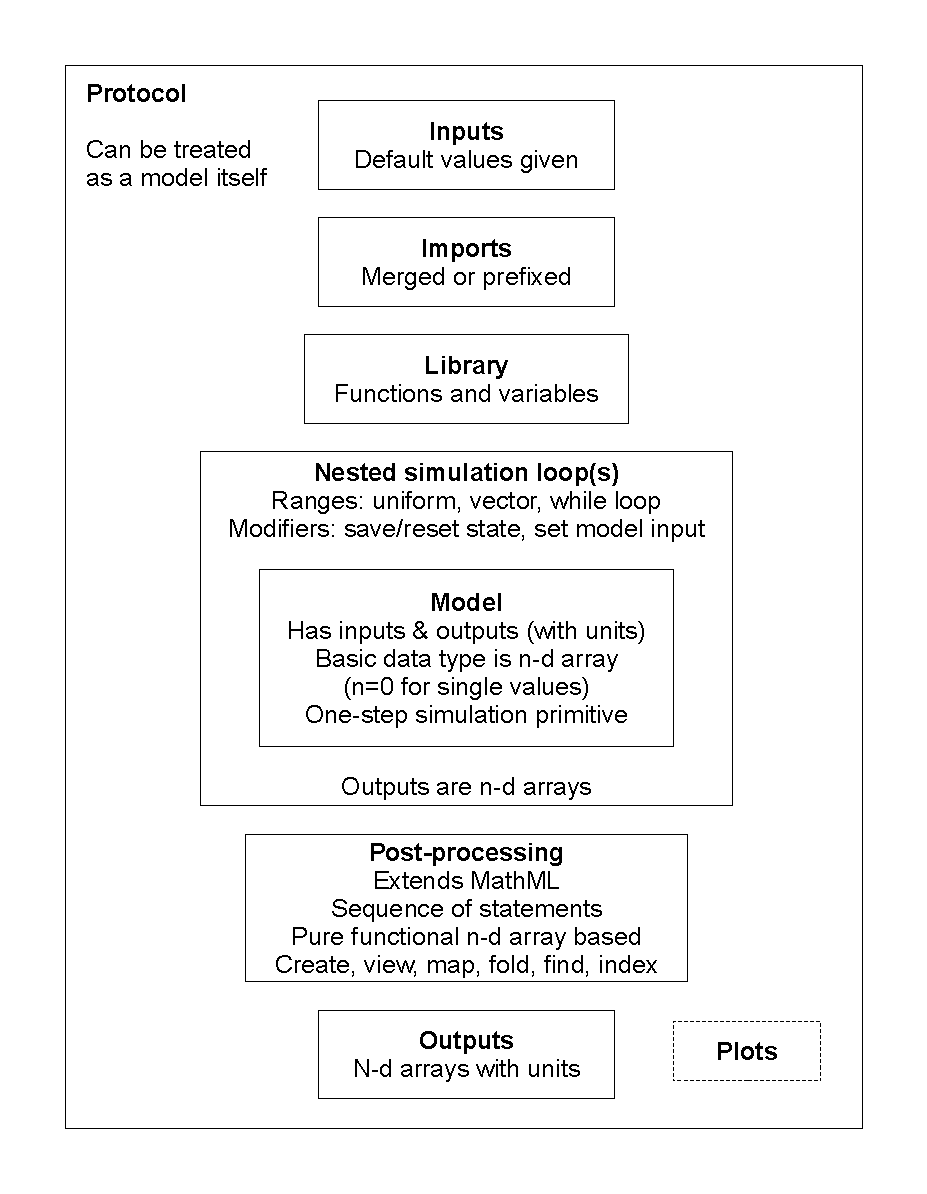
\includegraphics[height=.9\textheight]{proto_diag}
\end{center}
\end{frame}

\begin{frame}{Notes}
 * Further details on features, emphasis on what other kinds of protocol can be represented
 * Expressivity vs simplicity
 * Use flowcharts sent to Dave
 * Have a `describe your favourite protocol' challenge
 * Use some stuff from COMBINE talk: model interface, seq and nest sims, post-proc, libraries
\end{frame}

%%%%%%%%%%%%%%%%%%%%%%%%%%%%%%%%%%%%%%%%%%%%%%%%%%%%%%%%%%%%
\subsection{Interfacing protocols and models}

\begin{frame}{Interfacing protocols and models}
\begin{itemize}
\item Challenges arise from desire to apply a single experiment description to any model
  \subitem{And need to compare results for different models}
\item There are variations in modelling conventions
  \begin{itemize}
  \item Different names for the same `thing'
  \item Different ways of representing biology in mathematics
  \end{itemize}
\item An experiment may isolate a sub-component of the model (e.g.\ voltage clamp)
\end{itemize}
\end{frame}

\begin{frame}{Referring to model variables}
\begin{itemize}
\item How do we cope with different variable names for the same entity?
  \begin{itemize}
  \item Transmembrane potential: $V$, $V_m$, $E$
  \item Stimulus current: $i_{\mathrm{Stim}}$, $I_{\mathrm{st}}$, $i_{\mathrm{pulse}}$, $i_{\mathrm{ext}}$
  \item Membrane capacitance: $C$, $C_m$, $\mathit{Acap}$
  \end{itemize}
\item Use \alert{ontological annotation} of variables
\item Protocol can use \texttt{prefix:name} notation as for XML namespaces
\item No need for `approved' ontology --- just need model \& protocol to agree
\end{itemize}
\end{frame}

\begin{frame}{Units conversions}
\begin{itemize}
\item Different models use different units
\item Protocol declares the units it uses, and conversions applied automatically
  \note{This is easy for scalings within a dimension, but models can use different approaches to representing the same biology, e.g.\ different normalisation for ionic currents}
\item ``Biology-aware'' conversion rules can be defined
  \begin{itemize}
  \item A unary function for converting a value from one dimension to another
  \item Can refer to model variables using ontology terms
  \item Fall-back to next rule if required variables don't exist
  \item See also \doi{10.1016/j.pbiomolbio.2011.06.002}
  \end{itemize}
\end{itemize}
\end{frame}

\begin{frame}{Model modifications}
\begin{itemize}
\item A model is viewed as a \alert{system of equations}, independent of modelling language
\item<2-> Protocol specifies which variables are \alert{inputs} and \alert{outputs}
\item<2-> Inputs become parameters that can be set by the protocol
  \subitem{e.g.\ voltage clamp experiment}
\item<2-> Only those equations required for the given outputs need be computed
\item<3-> Equations may also be \alert{added or replaced}
  \subitem{e.g.\ to specify a stimulus current waveform}
\end{itemize}
\end{frame}

\begin{frame}{Interfacing protocols and models}
This will probably move, if we use it at all.
\begin{center}
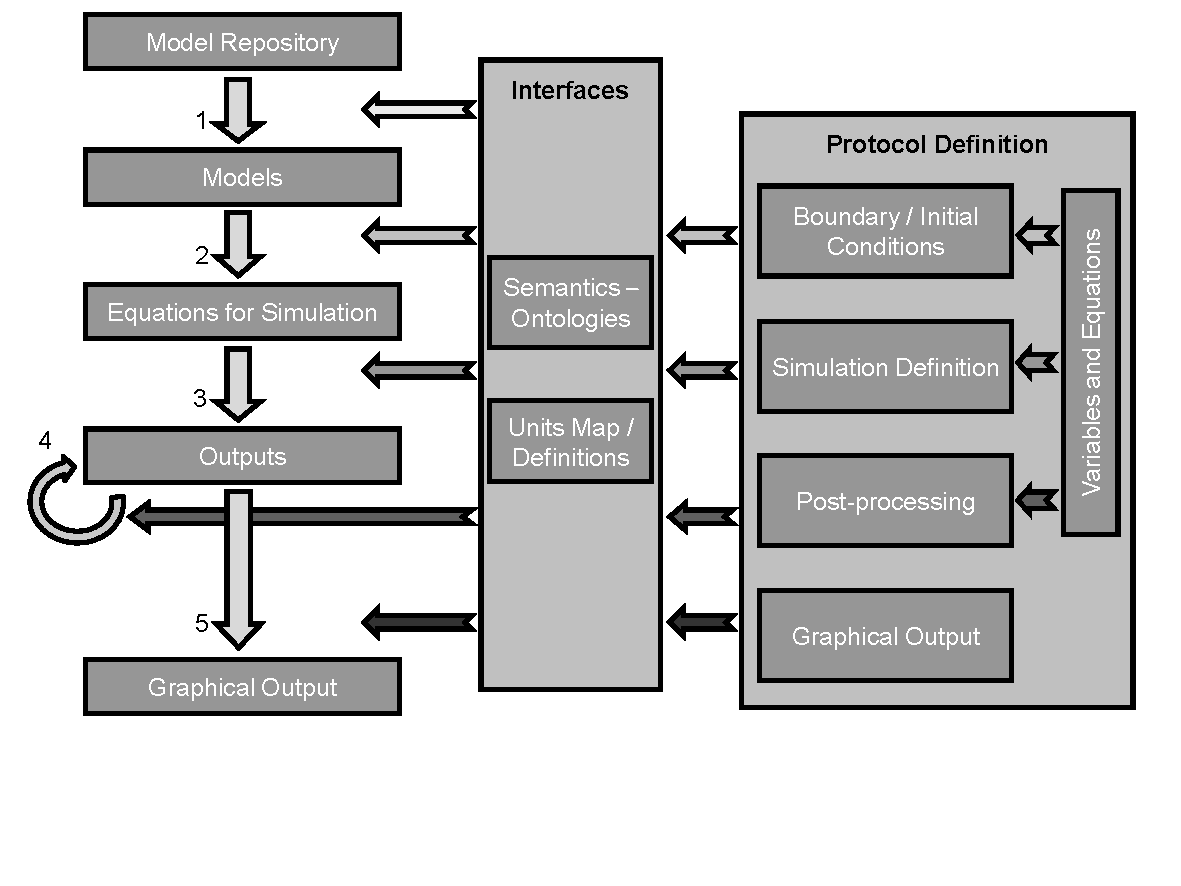
\includegraphics[width=.9\textwidth]{schematic_v4}
\end{center}
\end{frame}

%%%%%%%%%%%%%%%%%%%%%%%%%%%%%%%%%%%%%%%%%%%%%%%%%%%%%%%%%%%%
\subsection{Defining simulations}

\begin{frame}{Sequenced and nested simulations}
\begin{itemize}[<+->]
\item Basic simulation: timecourse solve of model equations
\item An experiment may have `setup' and `measurement' phases $\implies$ simulations should be able to run in sequence
\item \alert{Nesting} simulations supports parameter scans, repeated runs, distribution sampling, etc.
  \subitem{\alert{Model outputs therefore become regular $n$-dimensional arrays}}
\end{itemize}
\end{frame}

\begin{frame}{Simulation loops}
\begin{itemize}
\item Each simulation requires a \alert{range} over which to iterate for generating output points
\item These are given a name for the loop variable, and its units
  \begin{description}
  \item[\texttt{UniformStepper}] has start, stride, and end parameters
  \item[\texttt{VectorStepper}] allows irregular steps, using post-processing language constructs to define an array of values for the loop variable
  \item[\texttt{WhileStepper}] enables an outer loop to continue as long as a condition is met
  \end{description}
\end{itemize}
\end{frame}

\begin{frame}{Modifiers}
\begin{itemize}
\item Each simulation can also have a collection of \alert{modifiers}
  \begin{description}
  \item[SaveState] store the current model state, giving it a name
  \item[ResetState] reset the model to a stored state or initial conditions
  \item[SetVariable] set the value of a model variable\\
      The value is given by an expression in the post-processing language,
      and can access the current range value for this or any outer loop.
  \end{description}
\item Each can be applied just at the start or end of a simulation, or prior to each loop
\end{itemize}
\end{frame}

%%%%%%%%%%%%%%%%%%%%%%%%%%%%%%%%%%%%%%%%%%%%%%%%%%%%%%%%%%%%
\subsection{Post-processing}

% Slides from COMBINE:

\begin{frame}{Post-processing language}
\begin{itemize}
\item Aim to support complex operations with minimal implementation overhead
\item Therefore base on MathML, with as few as possible added \csym{csymbol}s
\item Key features:
  \begin{itemize}
  \item Operators for working with $n$-dimensional arrays
  \item Sequencing operations (assignments to variables, assertions)
  \item Defining functions (that can also be passed to other functions)
  \end{itemize}
\item Not just used for post-processing: also input specifications, library definitions, etc.
\item Technically, this is a pure functional $n$-dimensional array based programming language
\end{itemize}
\end{frame}

\begin{frame}{Main special expressions}
\footnotesize
\begin{description}
\item[\csym{newArray}] Create a new array
  \begin{itemize}
  \item by listing elements (which may be arrays)
  \item by \alert{comprehension} using a generator expression with index ranges
  (abusing \texttt{domainofapplication})
  \end{itemize}
\item[\csym{view}] Extract a sub-array
  \subitem{Can use arbitrary (even negative) strides over any dimension, with wildcards}
\item[\csym{map}] Map an $n$-ary function onto $n$ arrays element-wise
\item[\csym{fold}] Collapse an array along a single dimension using a binary function
  \subitem{Used to define \texttt{sum}, \texttt{max}, etc.}
\item[\csym{find}] Find indices where the operand array is non-zero
\item[\csym{index}] Create a sub-array containing only the given indices
  \subitem{Various options for avoiding irregular results}
\end{description}
\end{frame}

\begin{frame}{Statements}
\begin{itemize}
\item The \csym{statementList} is used for function bodies, and the library \& post-processing sections
\item 3 kinds of statement:
  \begin{itemize}
  \item Assignment: MathML \texttt{eq}
  \item Return: \csym{return} --- only valid in functions
  \item Assert: \csym{assert} --- for checking arguments etc.
  \end{itemize}
\end{itemize}
\end{frame}

\begin{frame}{Miscellaneous technicalities}
\begin{itemize}
\item Environments binding names to (immutable) values
\item Accessors (IS\_ARRAY, SHAPE, etc.)
\item Tuples
\item Default parameters
\item Wrapping MathML operators as functions
\item Location information for user-friendly error messages
\end{itemize}
\end{frame}

%%%%%%%%%%%%%%%%%%%%%%%%%%%%%%%%%%%%%%%%%%%%%%%%%%%%%%%%%%%%
\subsection{Other features}

\begin{frame}{Nested protocols}
\begin{itemize}
\item Since a protocol has inputs and outputs, it can be viewed as a kind of model
\item The ``system of equations'' abstraction does not apply, so model modifications are not possible
\item This does effectively allow us to interleave post-processing and simulation however
\item So we can do e.g.\ dynamic restitution without breaking the `regular $n$-d array' data model
\end{itemize}
\end{frame}

%%%%%%%%%%%%%%%%%%%%%%%%%%%%%%%%%%%%%%%%%%%%%%%%%%%%%%%%%%%%%%%%%%%%%%
\section{Conclusions and future directions}
\subsection*{Main}
%%%%%%%%%%%%%%%%%%%%%%%%%%%%%%%%%%%%%%%%%%%%%%%%%%%%%%%%%%%%%%%%%%%%%%

\begin{frame}{}
 * Caveats: usability, performance, still prototype; but lots of scope!
   * Example: FR00 APD
 * Conclusions and plans
\end{frame}

%%%%%%%%%%%%%%%%%%%%%%%%%%%%%%%%%%%%%%%%%%%%%%%%%%%%%%%%%%%%%%%%%%%%%%
\begin{frame}{Acknowledgments}
Gary Mirams, Chaste team, Alan Garny, Steven Niederer

\begin{center}

\includegraphics[scale=.9]{chaste-266x60}\\ \vspace{.4cm}

\includegraphics[width=.55\textwidth]{EPSRC1RGBLO} \hspace{.1cm}

\includegraphics[scale=.55]{logo_msr}
\end{center}
\end{frame}

\end{document}
